% !TEX TS-program = XeLaTeX
% محمود امین‌طوسی، بر اساس قالب CSICC2016 آقای دیانت
\documentclass{CCI2020}
\usepackage[utf8]{inputenc}
\usepackage{graphicx}
\usepackage{csquotes}
\usepackage{url}
\usepackage{fancyhdr}
\usepackage{float}
\floatplacement{figure}{H}


\pagestyle{empty}
\fancypagestyle{firstpage}{%
\fancyhf{}

\lhead{
\includegraphics[width=20mm]{images/AKUT.jpg}}

}
\renewcommand{\headrulewidth}{0.0pt}

% تقریبا تمامی بسته‌های مورد نیاز برای یک مقاله در استایل فراخوانی شده است. اما در هر صورت در صورتی‌که می‌خواهید بسته‌ای را فراخوانی کنید به صورت زیر عمل کنید. مثلا ما در کد زیر دوبسته glossaries و tikz را فراخوانی کرده‌ایم.
%\makeatletter
%\bidi@BeforePackage{xepersian}{
%\RequirePackage{tikz}
%\RequirePackage{glossaries}
%}
%\makeatother


% عنوان مقاله را در این قسمت وارد کنید. 
\title{
سیستم هوشمند پرسش و پاسخ مبتنی بر ویکی‌پدیا در حوزه‌ی پزشکی
}
\date{}
% اسامی نویسندگان و همچنین اطلاعات مربوط به آن‌ها را در این قسمت وارد کنید. 
\author{غزاله خرادپور}
\affil{
 دانشجوی کارشناسی رشتهٔ علوم کامپیوتر، دانشکدهٔ علوم کامپیوتر دانشگاه صنعتی امیرکبیر، تهران، ایران
}
\affil{
استاد راهنما: دکتر اکبری
}


\begin{document}
\maketitle
\thispagestyle{firstpage}
\begin{abstract}
در این پروژه، سعی بر آن بود که با وجود سیستم پرسش و پاسخ مبتنی بر مقاله‌های ویکی‌پدیای\footnote{Wikipedia} غیرفارسی، داده‌هایی به زبان فارسی -چه به صورت اتوماتیک و چه به صورت دستی- جمع‌آوری شود و سپس به کمک سیستم‌های هوشمند موجود، سیستمی پیاده‌سازی کنیم که کاربران بتوانند با وارد کردن سؤالات پزشکی خود به زبان فارسی، پاسخی درخور همان سوال به همان زبان فارسی دریافت کنند.
 \end{abstract}
\begin{keywords}
سیستم پرسش و پاسخ، ویکی‌پدیا، پزشکی، دیتا، اتوماتیک، پردازش زبان طبیعی
\end{keywords}


\section{مقدمه}
پرسش و پاسخ یک زمینهٔ تحقیقاتی در رشتهٔ علوم کامپیوتر و در حوزهٔ بازیابی اطلاعات و پردازش زبان طبیعی\footnote{NLP} است که هدف از آن طراحی سیستم‌هایی است که به‌طور خودکار به سوالات مطرح شده توسط انسان در ساختار زبان طبیعی پاسخ تولید می‌کند. پیاده‌سازی سیستم پرسش و پاسخ، معمولاً به‌صورت یک برنامهٔ رایانه‌ای است که پاسخ‌های خود را با پرس‌و‌جو از یک پایگاه دادهٔ ساخت‌یافته از دانش یا اطّلاعات، معمولاً یک پایگاه دانش ایجاد می‌کند. به طور معمول، سیستم‌های پرسش و پاسخ می‌توانند پاسخ‌ها را از یک مجموعهٔ بدون ساختار از اسناد زبان طبیعی دریافت کنند.
از سری اسناد زبان طبیعی که برای دریافت جواب سؤالات از آن استفاده می‌شود، می‌توان به مجموعه‌ای محلّی از متون مرجع
اسناد و صفحات وب سازمان داخلی،
گزارش‌های خبری خبرگزاری‌ها،
مجموعه‌ای از صفحات ویکی‌پدیا و 
زیرمجموعه‌ای از صفحات وب جهانی اشاره کرد.
برای دریافت جواب‌ها از اسناد دو نوع منبع دامنه‌محدود و دامنه‌باز وجود دارد که هر کدام شرایطی دارند و انتخاب ما اسناد دامنه‌محدود بوده است به این معنی که با یک دامنهٔ خاصّی از موضوعات سروکار دارند و موضوع مورد نظر ما حوزهٔ پزشکی بوده است. در آینده آن را به دامنه‌باز تبدیل خواهیم کرد.



حال سیستم پرسش و پاسخ هوشمند در حوزهٔ پزشکی می‌تواند کمک بزرگی برای کاربران باشد از آن جا که پزشک و اطّلاعات پزشکی در اختیار تمام مردم نیست و حتّی اگر در دسترس هم باشد، ممکن است در یافتن جواب‌های خود دچار گمراهی شوند. افراد با حلّ مشکلات پزشکی سطحی خود، امکانات محدود پزشکی را در اختیار افرادی قرار می‌دهند که به آن نیاز شدیدی دارند.
از طرفی جواب دادن به سؤالات پزشکی نیازمند دانستن دانش بسیار است و هر فردی در شرایط عادی آن‌ها را نمی‌داند و وقت زیادی ندارد تا منابع مختلف را مطالعه کند، این سیستم می‌تواند بسیار کمک‌کننده باشد. علاوه بر این پزشکان نیز می‌توانند صحّت تشخیص و دانسته‌های خود را از این طریق تثبیت کنند و دانش پزشکی و ارتباط با بیماران به سمت هوشمندتر شدن می‌رود.
بنابراین سیستمی که بتواند به پرسش‌های کاربران پاسخ مناسب برگرداند، بسیار خدمت بزرگی است و برای آن‌ها کم‌هزینه است. تنها با وارد کردن سوالات خود به زبان طبیعی، به جواب متناسب می‌رسند.

ما برای پیدا کردن جواب سؤالات پاسخ‌بلند خود از ویکی‌پدیا به عنوان منبع دایرة‌المعارف‌گونه استفاده می‌کنیم. ویکی‌پدیا منبع قدرتمندی است که اطّلاعات به‌روزی دارد و هر روز بهتر می‌شود؛ چون توسّط عدّهٔ زیادی از مردم نوشته و ویرایش می‌شود، کم‌تر حاوی اطّلاعات غلط است و می‌توان سیستم‌های هوشمندی روی آن پیاده کرد.



\begin{figure*}[!htp]
    \centering
    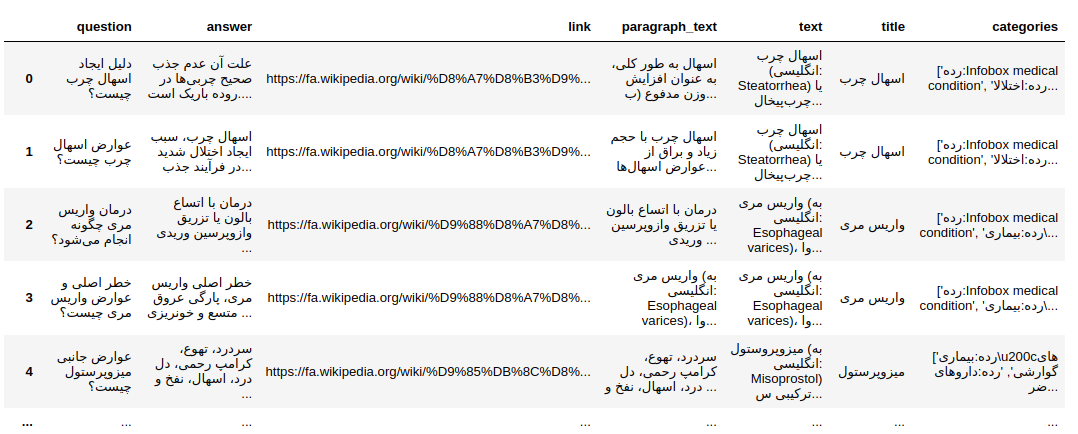
\includegraphics[width=15cm]{images/data.png}
    \caption{نمونه‌ای از دادهٔ جمع‌آوری‌شده}
    \label{fig:data}
\end{figure*}


\section{منابع داده}
منابع اصلی ما داده‌های تمامی صفحات ویکی‌پدیا و داده‌های جمع‌آوری‌شده بودند که از داده‌های ویکی‌پدیا به عنوان منبعی برای استخراج جواب استفاده می‌کنیم و از داده‌های جمع‌آوری‌شده برای آموزش دادن مدلی که قادر است بهترین جواب برای سوّال پرسیده‌شده را برگرداند.
چالش اصلی کار ما، پیدا کردن دادهٔ مناسب به زبان فارسی بود و از آن جا کار مشابهی قبلاً به زبان فارسی انجام نشده است و به طور کلّی در پردازش زبان طبیعی به فارسی پیشینهٔ خاصّی وجود ندارد، دادهٔ مناسبی هم در اختیار نداشتیم. چندین منبع برای این نوع مجموعه‌داده‌ها وجود داشتند که هم محدود بودند و هم ساختاری به شکل آن چه ما می‌خواستیم نداشتند. کاری که ما می‌خواستیم انجام دهیم، چون پردازش زبان طبیعی بود و باید از گونه‌ای از شبکهٔ عصبی بهره می‌گرفتیم، به دیتای بسیار زیادی برای آموزش نیاز داشتیم تا به هدفی که برای خود تعیین کرده بودیم، برسیم.

\begin{figure*}[!htp]
    \centering
    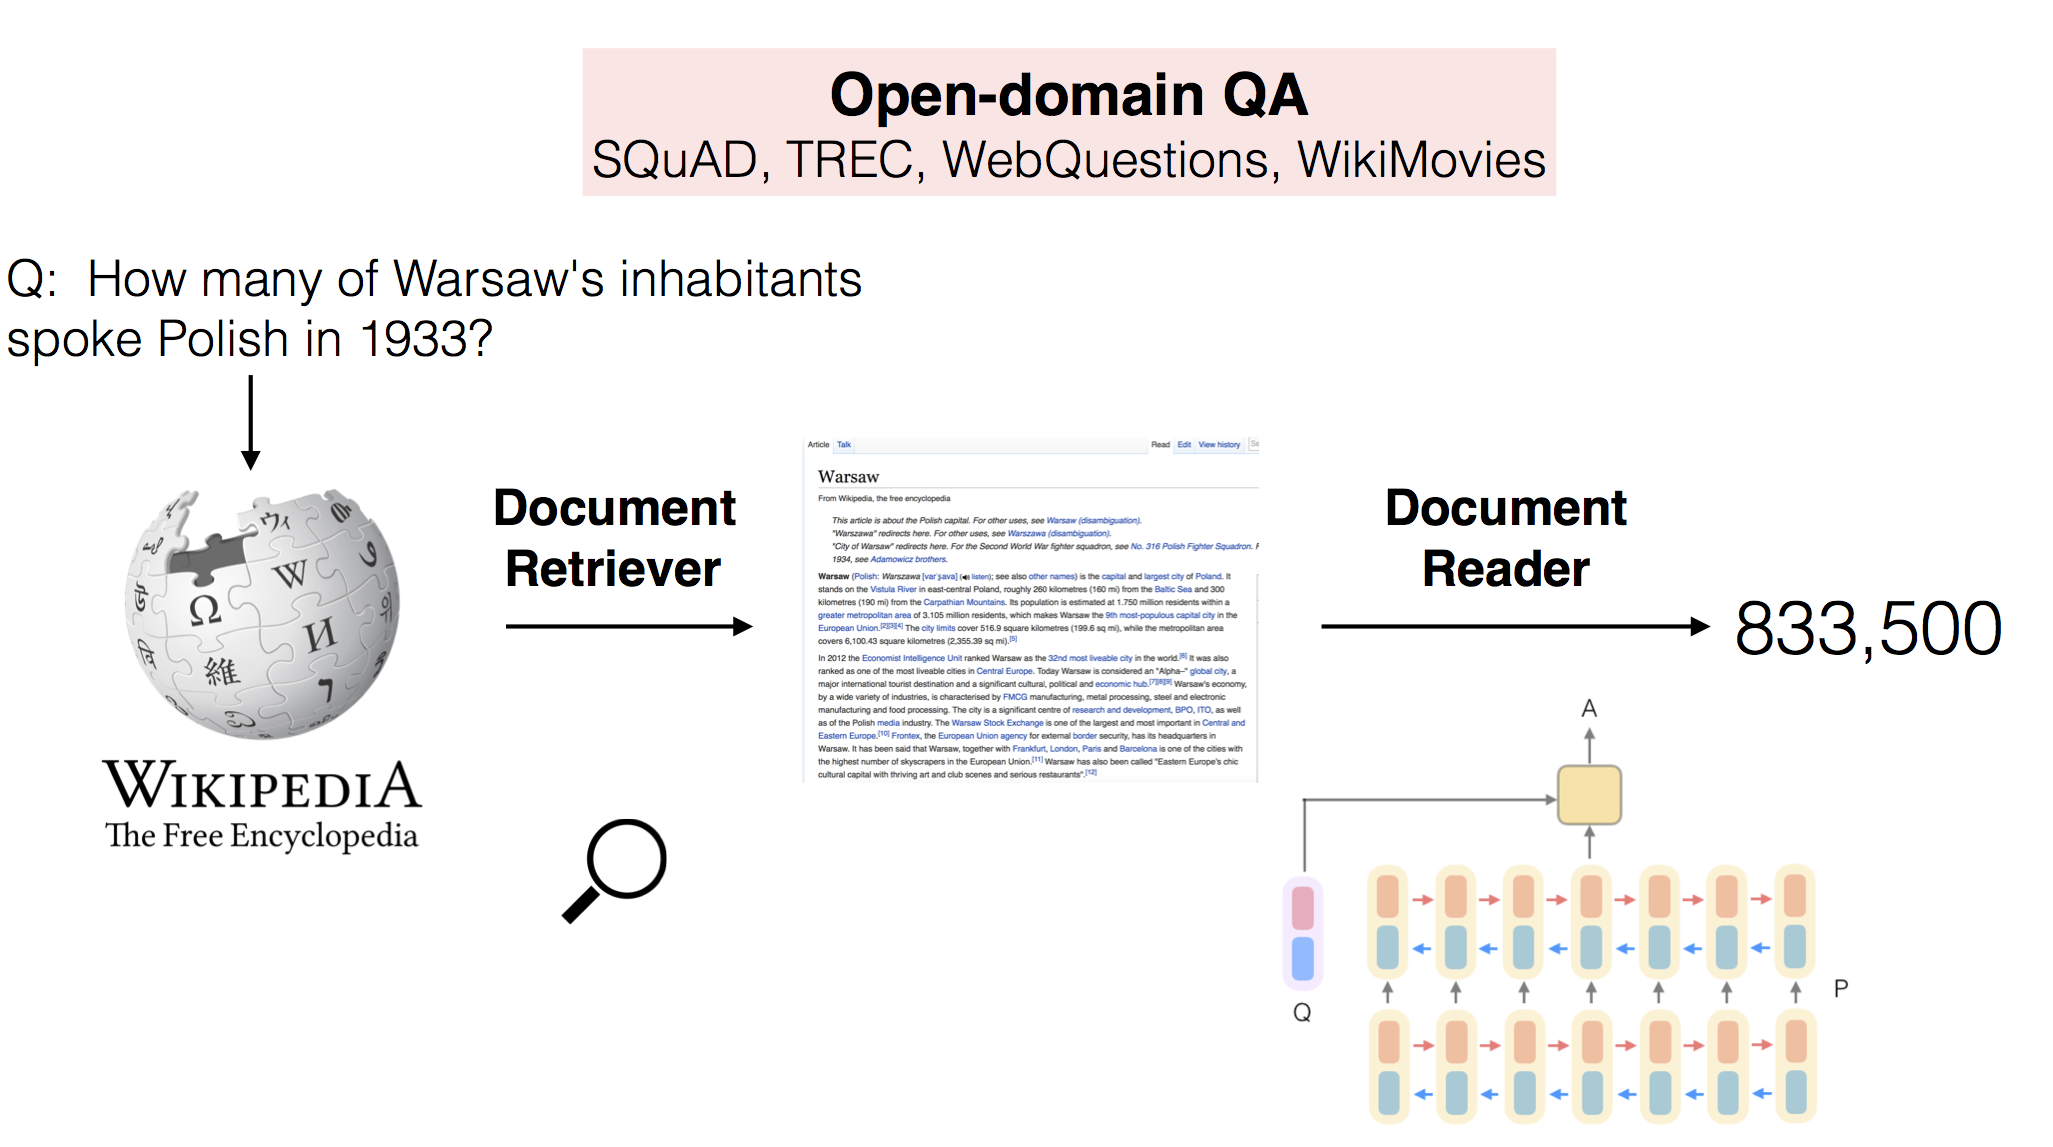
\includegraphics[width=15cm]{images/drqa.png}
    \caption{شیوهٔ کار سیستم \lr{DrQA}}
    \label{fig:drqa}
\end{figure*}


\subsection{ویکی‌پدیا}
از ویکی‌پدیا به عنوان منبع دانش استفاده می‌شود. حال
برای استخراج تمامی مقالات ویکی‌پدیا باید حدود ۵ میلیون صفحه استخراج شود و تمامی شکل‌ها و ساختارهای مربوطه از بین برود و فقط متن به تنهایی در نظر گرفته و ذخیره شود.



\subsection{مجموعه‌داده‌های جمع‌آوری‌شده}
برای این که بتوانیم مدلی آموزش دهیم تا نتیجهٔ نزدیک به مطلوب را به ما بدهد، نیاز به داده‌های بسیار زیادی از زبان فارسی داشتیم و از آن جا که مجموعه‌داده‌ها -خصوصاً در حوزهٔ پزشکی- بسیار کم بود، شروع به جمع‌آوری هزار ردیف دادهٔ فارسی -با این که باز هم مقدارش کم بود- کردیم. این دیتاها به صورت دستی از سایت ویکی‌پدیا استخراج شدند و ستون‌های آن شامل سؤال، جواب، متن پاراگراف (زمینه\footnote{context})، تیتر مقاله و متن کل مقاله است. از متن پاراگراف و کلّ مقاله برای یاد دادن نحوهٔ استخراج جواب از زمینه به ماشین استفاده می‌کنیم.  داده‌ها دارای ساختاری به شکلی زیر هستند:
\begin{itemize}
    \item سؤال: سؤالی بر اساس مطلب موجود در ویکی‌پدیا طرح شده است.
    \item جواب: جواب سؤال طرح‌شده به صورت عینی از قسمتی از پاراگراف‌های یکی از مطالب ویکی‌پدیا  نوشته شده است.
    \item زمینه: پاراگرافی که از آن جواب استخراج شده، ذخیره شده است. این ستون از داده‌ها برای آموزش مدل بسیار حائز اهمیّت است.
    \item تیتر: تیتری مطلبی از ویکی‌پدیا که سؤال و جواب از آن گرفته شده است.
    \item متن کل: متن تمام مقالهٔ مورد نظر در ویکی‌پدیا ذخیره شده است.
    \item رده‌ها: رده‌هایی که در قسمت پایینی صفحهٔ ویکی‌پدیا به صورت لیستی قرار داده شده‌اند، ذخیره شده است.
\end{itemize}

لازم به ذکر است که سه مورد انتهایی مجموعه‌داده‌ها به صورت اتوماتیک و با استفاده از کد استخراج شده است. نمونه‌ای داده‌ها در شکل \ref{fig:data} آمده‌اند




\subsection{مجموعه‌داده‌های ترجمه‌شده}
از آن‌جا داده‌های جمع‌آوری شده به صورت دستی کافی نبودند، شروع به ترجمهٔ مجموعه‌دادهٔ \lr{SQuAD} \cite{ref2} کردیم و با این که تقریباً ربط زیادی به حوزهٔ پزشکی نداشتند و \lr{API} سیستم مترجم گوگل\footnote{Translate Google} قادر به ترجمهٔ تمام و کمال مجموعه‌داده‌ها نبود، این داده‌ها هم بلااستفاده ماندند و در مراحل بعدتر و برای بهتر کردن مدل آموزش‌داده‌شده به ماشین از آن‌ها استفاده خواهیم کرد. علاوه بر خود مجموعه‌داده‌های این مجموعه، ستون‌هایی به آن‌ها اضافه کردیم که شامل ترجمه‌هایی به زبان فارسی هستند و سوال، جواب، تیتر مقاله و زمینه به زبان فارسی ترجمه شده‌اند.


\section{مروری بر کارهای پیشین}
برای سیستم پرسش و پاسخ به زبان فارسی، هیچ کاری انجام نشده است چون همان‌طور که قبلاً اشاره کردیم، مشکل کمبود داده و پیچیدگی‌های زبان فارسی چالش‌های زیادی را ایجاد می‌کند. به زبان‌های دیگر خصوصاً انگلیسی کارهای زیادی انجام شده است.

کارهای مشابه دیگری به عنوان مثال توسّط \lr{. Ryu et al.} \cite{ref3} انجام شده است که سیستم پرسش و پاسخ دامنه‌بازی طرّاحی کرده است که از ویکی‌پدیا به عنوان منبع مدل خود استفاده می‌کند و متن مقاله‌ای را با جواب‌های منطبق دیگر مانند جعبه‌های اطّلاعات \footnote{infoboxes}، ساختار مقاله، ساختار دسته‌بندی و تعاریف ترکیب می‌کند. به طور مشابه \lr{Ahn et al.} \cite{ref4} هم که از ویکی‌پدیا به عنوان منبع متن با ترکیب دیگر منابع استفاده می‌کند.
علاوه بر آن، \lr{Buscaldi and Rosso} \cite{ref5} از ویکی‌پدیا به عنوان منبع دانش خود استفاده می‌کند امّا به جای آن که جواب‌ها را از روی آن بیابد، از آن برای ارزیابی کردن جواب تولید‌شده توسّط خود سیستم استفاده می‌کند و از دسته‌بندی‌های ویکی‌پدیا برای اطمینان از مجموعه الگوهایی که برای جواب پیش‌بینی‌ شده، بهره می‌برد.

سیستم‌های پیشرفته‌تری از پرسش و پاسخ وجود دارند که از ویکی‌پدیا و وب استفاده می‌کنند؛ مانند \lr{QuASE}، \lr{Microsoft's AskMSR} \cite{ref6}،  \lr{IBM's DeepQA} و YodaQA \cite{ref7} که هر کدام از روش‌های خاصّ خود برای پیاده‌سازی این سیستم استفاده کرده‌اند.


\begin{figure*}[t]
  \begin{minipage}[t]{\linewidth}
    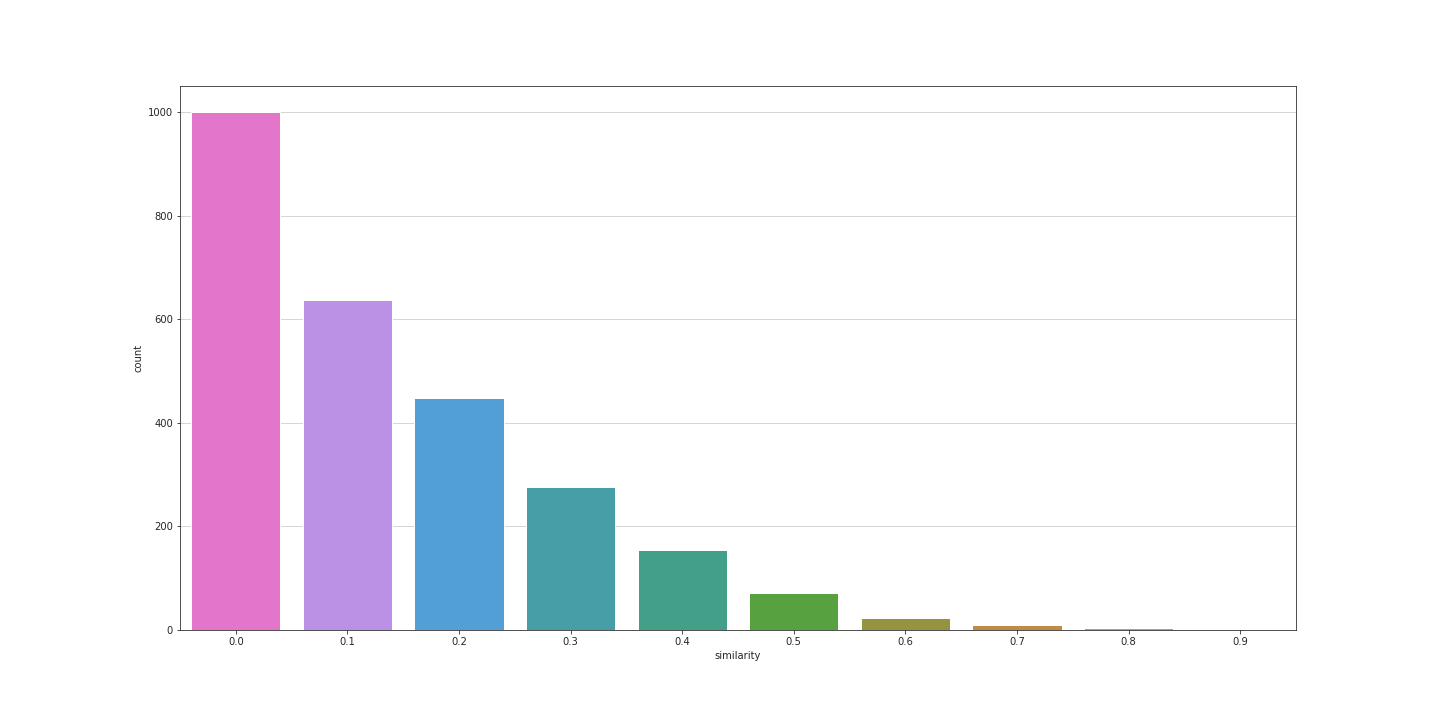
\includegraphics[width=\linewidth]{images/similarity_count.png}
    \caption{شباهت بین سؤال‌ها و جواب‌های یک ردیف در دادهٔ جمع‌آوری‌شده}
    \label{fig:sim}
  \end{minipage}\hfill%
\end{figure*}




که یکی از بزرگ‌ترین و مشابه‌ترین کارها به کار ما، پروژه‌ای به نام \lr{DrQA}\cite{ref1}
است و کاری را انجام داده است که برنامه داشتیم انجام دهیم. بدنهٔ این پروژه به گونه‌ای است که با وارد کردن دادهٔ فارسی می‌توان مدلی را آموزش داد و از نتیجهٔ آن استفاده کرد. شکل کلّی این پروژه در شکل \ref{fig:drqa} نشان داده شده است.


\subsection{\lr{DrQA} چیست؟}
ک سیستم درک مطلب از طریق خواندن است که از ویکی‌پدیا به عنوان تنها منبع خود برای یافتن جواب استفاده می‌کند به طوری که انگار شخصی از روی دایرة‌المعارف جواب سؤالات را می‌دهد. البتّه این سیستم به گونه‌ای طرّاحی شده است که می‌توان هر منبعی را به عنوان منبع پیدا کردن جواب سؤالات برای آن انتخاب کرد و قابلیّت مقیاس‌پذیری دارد. این سیستم پس از دریافت سؤال، به دنبال جوابی برای آن سؤال می‌گردد. تمرکز این پروژه بر روی سؤال و جواب‌های طولانی (نه یک کلمه‌ای) است و در این مسیر با چالش‌هایی هم‌چون پیدا کردن مقاله‌های مرتبط و پیدا کردن جواب از روی آن‌ها دست و پنجه نرم می‌کند. این پروژه از ویکی‌پدیای انگلیسی -از آن جا که بسیار غنی و باجزییات است- به عنوان منبع جواب‌های خود استفاده می‌کند.

\lr{DrQA} از دو قسمت اصلی تشکیل شده است که قسمت اوّل آن تمام مقالات ذخیره‌شده را می‌خواند و از بین آن ۵ مقاله‌ای پتانسیل دارا بودن جواب را در خود دارند، بر می‌گرداند و قسمت دوّم آن همان هستهٔ اصلی است که مدل روی آن آموزش دیده است.



این پروژه از شبکهٔ عصبی مکرر چندلایه\footnote{\lr{multi-layer recurrent neural network machine comprehension}} که در حالت پیش‌فرض روی مجموعه‌داده‌های SQuAD آموزش داده شده است، به عنوان پردازش‌کنندهٔ مطالب استفاده می‌کند و در نهایت جواب‌های منتخب را با امتیاز حساب شده توسط مدل ارائه می‌دهد و بهترین آن را به عنوان جواب برمی‌گرداند.

\begin{itemize}
    \item \lr{Document Retriever}: 
 تمام داده‌ها و مقالات ویکی‌پدیا به صورت ماتریس‌های وزن‌داده‌شده \lr{TF-IDF} ذخیره می‌شوند. پس از آن که سؤال دریافت شد، توسط ادغام \lr{TF-IDF} و \lr{n-grams} -حتّی سریع‌تر و با دقّت بهتر از موتور جست‌وجوی خود ویکی‌پدیا- مقالات مرتبط را پیدا می‌کند.
 
 \item \lr{Document Reader}: پس از کدگذاری پاراگراف‌ها (با استفاده از الگوریتم \lr{LSTM}\footnote{\lr{long short term memory}})، استفاده از شبکهٔ عصبی مکرّر چندلایه کدگذاری سؤال و کدگذاری متن سؤال، جواب منتخب را از بین پاراگراف‌های مقالات منتخب مرحلهٔ قبل حدس می‌زند.
\end{itemize}

% \begin{figure*}[H]
%     \centering
%     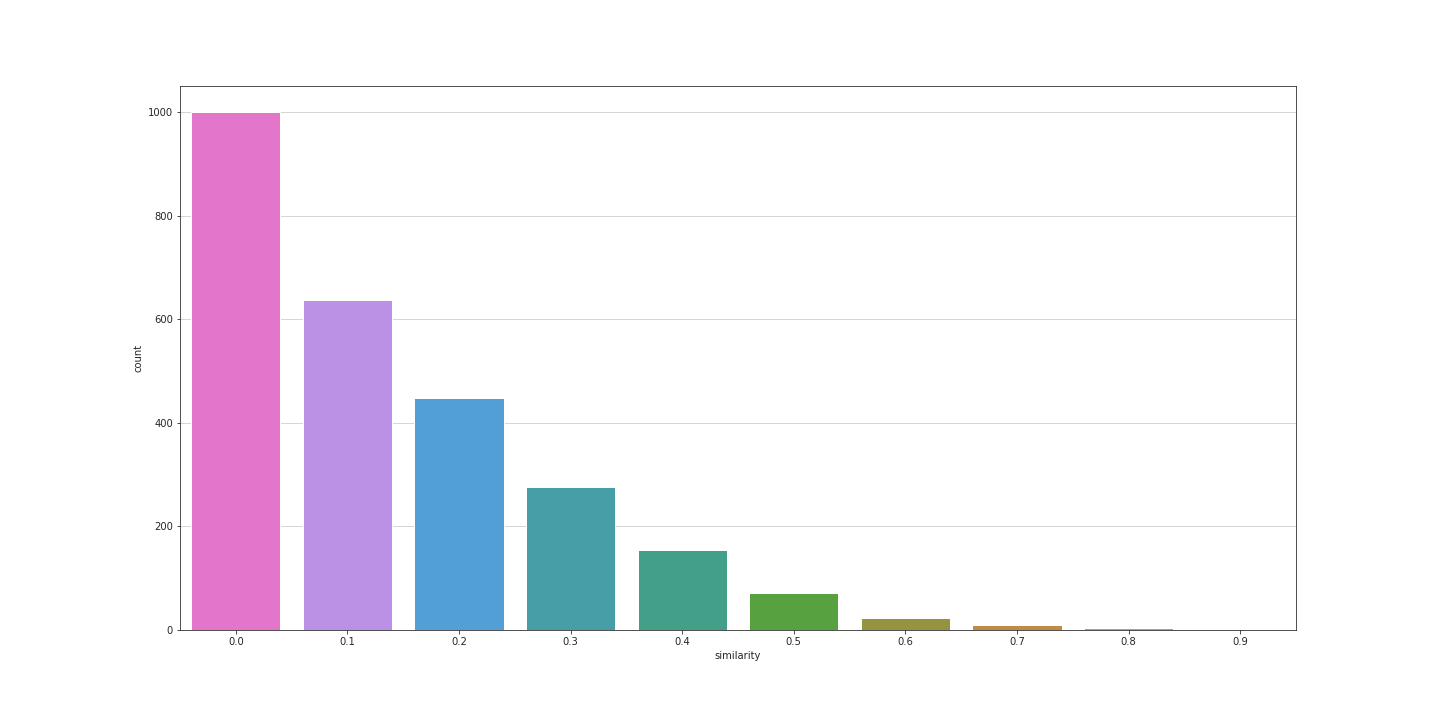
\includegraphics[width=18cm]{images/similarity_count.png}
%     \caption{شباهت سؤال و جواب هر ردیف داده }
%     \label{fig:sim}
% \end{figure*}






\section{پیش‌پردازش‌های انجام‌شده روی داده‌ها}
بخش اعظم این پروژه جمع‌آوری داده‌ها بوده است که برای درک بهتر ساختارها و اجزای آن یک سری پیش‌پردازش‌ها انجام داده‌ایم تا بدانیم با چه جنس داده و با چه توزیعی از کلمات مواجه هستیم. یکی از کارهای اصلی‌ای که برای پیش‌پردازش داده‌ها در فرآیند پردازش زبان طبیعی انجام می‌شود، حذف کلمات کلیدی \footnote{stopwords} است که انجام دادن آن در این پروژه بی‌معنی است. تنها کلمات غیرفارسی را از آن حذف کردیم و الگوهای زبانی را در آن بهبود بخشیدیم. دو نمونه از آمارهایی که در مورد مجموعه‌داده‌ها رسم کرده‌ایم، در شکل \ref{fig:wc} و \ref{fig:sim} آمده‌اند.

برای این که ارتباط بین سؤالات و جواب‌های هر ردیف از داده‌ها را بدانیم، با استفاده از روش \lr{TF-IDF} متن سؤال‌ها و جواب‌ها به بردار تبدیل کردیم و سپس با روش \lr{Cosine Similarity} شباهت بین سؤال‌ها و جواب‌های هر ردیف را بررسی کردیم. سؤال‌ها و جواب‌ها تا حدی خوبی به هم شبیه بودند و ارتباط بین‌شان مشهود بود از آن جا امتیاز شباهتشان با روش مذکور، به طور متوسط روی ۰/۳ بود و این عدد نسبتاً خوبی است.

% \begin{figure}[!htp]
%     \centering
%     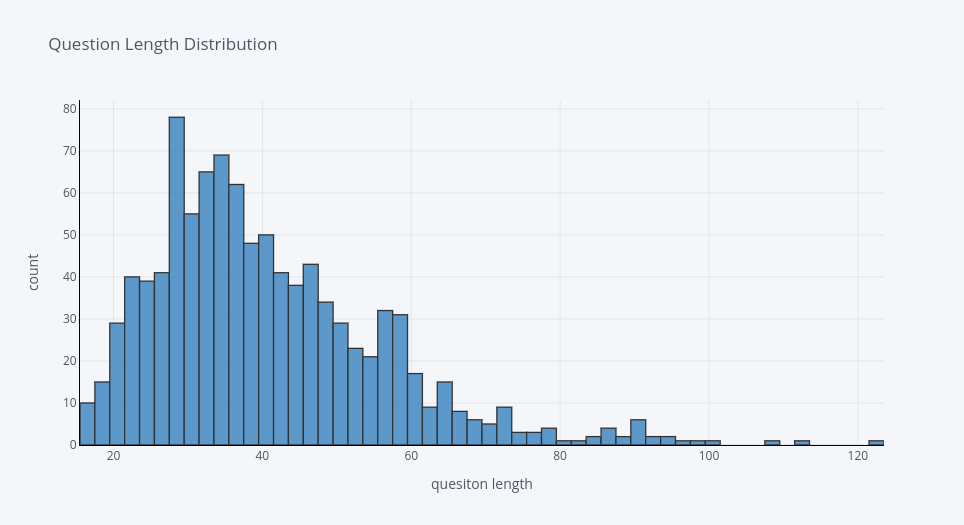
\includegraphics[width=10cm]{images/newplot (1).png}
%     \caption{توزیع طول سؤالات مجموعه‌دادهٔ جمع‌آوری‌شده}
%     \label{fig:galaxy}
% \end{figure}

\begin{figure}[H]
    \centering
    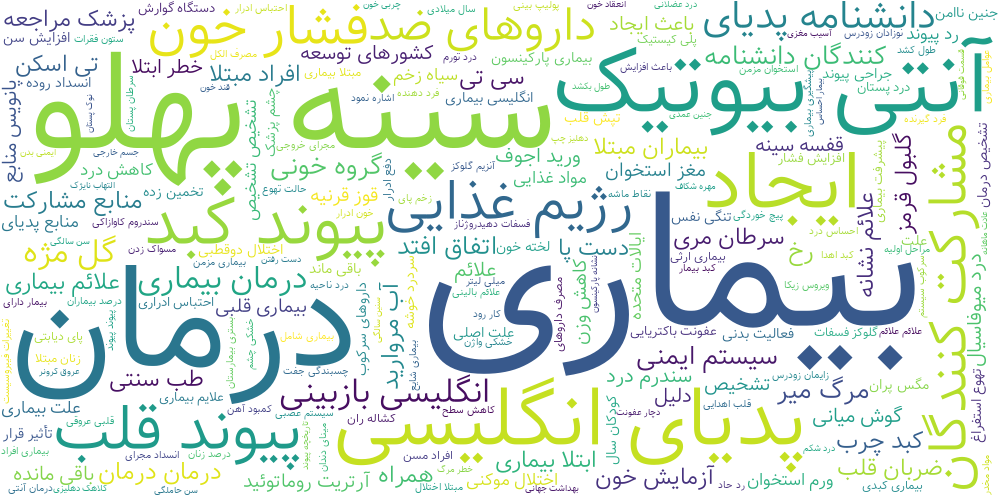
\includegraphics[width=\linewidth]{images/wordcloud.png}
    \caption{ابر کلمات استفاده شده در متن‌های مجموعه‌داده‌های جمع‌آوری‌شده}
    \label{fig:wc}
\end{figure}

\section{نتیجه}
این پروژه با بیشتر شدن داده‌ها، به امتیاز بیشتری خواهد رسید و هدف ما این است که این پروژه را در زمینه‌های دیگری به غیر از پزشکی نیز گسترش دهیم و در مراحل بعدتر به الگوریتم‌های موجود در این زمینه بهبود بخشیم.
\\
\\
\\


%\bibliographystyle{ieeetr-fa}

\bibliography{lib}

\end{document}


